\documentclass[aspectratio=169,12pt]{beamer}
\usepackage{amsmath}
\usepackage{amssymb}
\usepackage{xcolor}
\usepackage[most]{tcolorbox}
\usepackage{graphicx}
\usepackage[sfdefault,lf]{FiraSans}
\renewcommand{\familydefault}{\sfdefault}
\setlength{\parindent}{0pt}
\everymath{\displaystyle}
\setbeamertemplate{navigation symbols}{}
\setbeamertemplate{footline}{}
\setbeamertemplate{headline}{}
\definecolor{mmpageWhite}{HTML}{FCFBF7}
\definecolor{mmtanSoft}{HTML}{F7F5EF}
\definecolor{mmgreenDeep}{HTML}{244B2C}
\definecolor{mmgreenLeaf}{HTML}{5D8A56}
\definecolor{mmtext}{HTML}{163221}
\definecolor{mmanswerColor}{HTML}{306A3A}
\setbeamercolor{background canvas}{bg=mmpageWhite}
\setbeamercolor{normal text}{fg=mmtext,bg=mmpageWhite}
\newtcolorbox{MMProblemCard}[1][]{enhanced,breakable=false,colback=white,colframe=black,boxrule=1.0pt,arc=5pt,left=3pt,right=3pt,top=2pt,bottom=2pt,before skip=0pt,after skip=0pt,height=0.22\textheight,valign=top,#1}
\newcommand{\KoruIcon}{\raisebox{-0.2em}{
\includegraphics[height=1.05em]{img/header-logo.png}}}
\newcommand{\HoeIcon}{\raisebox{-0.2em}{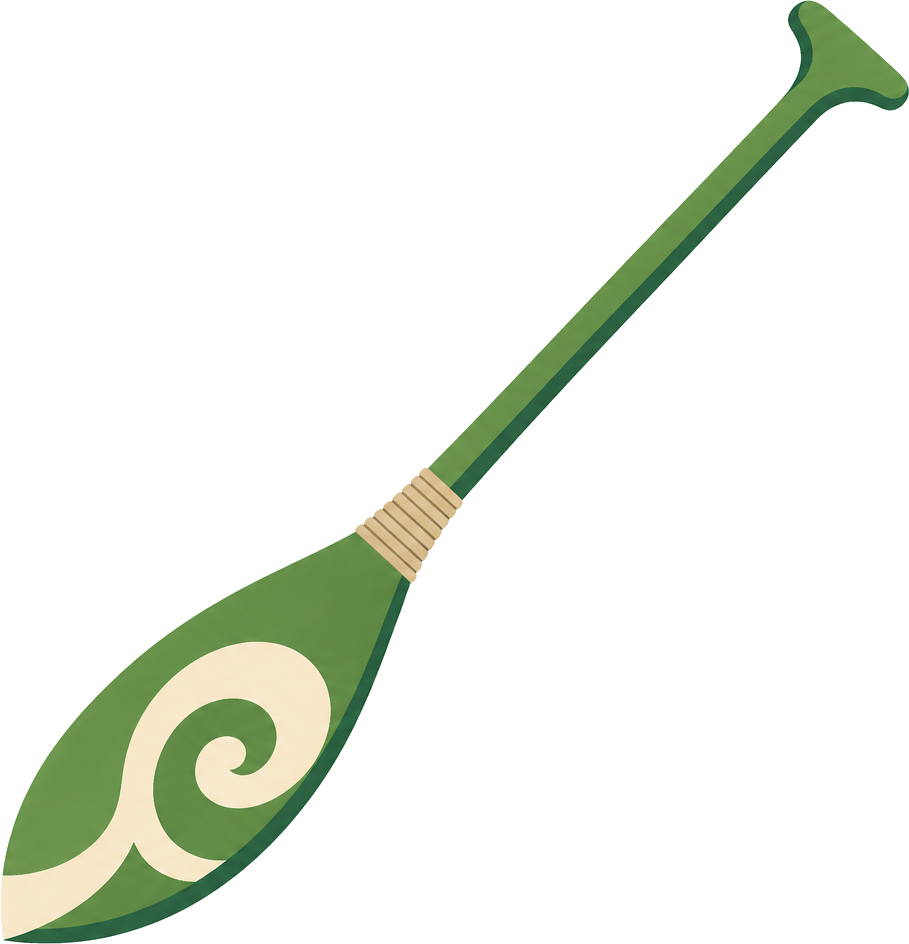
\includegraphics[height=1.05em]{img/hoe.png}}}
\newcommand{\ScaffoldIcons}[1]{\ifcase#1\or \HoeIcon\or \HoeIcon\hspace{0.22em}\HoeIcon\or \HoeIcon\hspace{0.22em}\HoeIcon\hspace{0.22em}\HoeIcon\fi}
\newcommand{\WorksheetTitle}[2]{%{
  \colorbox{mmtanSoft}{\parbox[c][2.0em][c]{0.975\linewidth}{\hspace{0.25em}{\Large\bfseries\textcolor{mmgreenDeep}{#1}\hfill\ScaffoldIcons{#2}}}}
  \par\vspace{0.08em}{\color{mmgreenLeaf}\rule{\linewidth}{2.0pt}}\par\vspace{0.04em}}
\newcommand{\MMAnswer}[2]{\begin{MMProblemCard}\raggedright\small\textbf{#1.} \textcolor{mmanswerColor}{\textbf{#2}}\par\end{MMProblemCard}}
\setbeamertemplate{background}{\begin{tikzpicture}[remember picture,overlay]\draw[black,line width=1.5pt,rounded corners=10pt]([xshift=0.45cm,yshift=-0.45cm]current page.north west) rectangle ([xshift=-0.45cm,yshift=0.45cm]current page.south east);\end{tikzpicture}}
\begin{document}

\begin{frame}[t]
\WorksheetTitle{Push Tasks - Answers}{3}
\vspace{-0.18em}
\begin{columns}[T,onlytextwidth]
\begin{column}{0.32\textwidth}\MMAnswer{1}{1 = $\angle BAE$ or $\angle EAB$}\end{column}
\begin{column}{0.32\textwidth}\MMAnswer{2}{2 = $\angle EAD$ or $\angle DAE$; 3 = $\angle DAC$ or $\angle CAD$; 4 = $\angle CAP$ or $\angle PAC$}\end{column}
\begin{column}{0.32\textwidth}\MMAnswer{3}{$\angle QPT$ = 1+2+3}\end{column}
\end{columns}
\vspace{0.45em}
\begin{columns}[T,onlytextwidth]
\begin{column}{0.32\textwidth}\MMAnswer{4}{$\angle RPS$ = 3+4; $\angle TPQ$ = 1+2+3; $\angle SPQ$ = 1+2}\end{column}
\begin{column}{0.32\textwidth}\MMAnswer{5}{$\angle ACB$}\end{column}
\begin{column}{0.32\textwidth}\MMAnswer{6}{$\angle DFE$ or $\angle EFD$}\end{column}
\end{columns}
\vspace{0.45em}
\begin{columns}[T,onlytextwidth]
\begin{column}{0.32\textwidth}\MMAnswer{7}{$\angle HGI$ or $\angle IGH$}\end{column}
\begin{column}{0.32\textwidth}\MMAnswer{8}{$\angle MLN$ or $\angle NLM$}\end{column}
\begin{column}{0.32\textwidth}\MMAnswer{9}{$\angle NLM$ or $\angle MLN$}\end{column}
\end{columns}
\end{frame}

\begin{frame}[t]
\WorksheetTitle{Push Tasks - Answers}{3}
\vspace{-0.18em}
\begin{columns}[T,onlytextwidth]
\begin{column}{0.32\textwidth}\MMAnswer{10}{1+2+3+4+5}\end{column}
\begin{column}{0.32\textwidth}\MMAnswer{11}{3+4+5; 1; 2+3}\end{column}
\begin{column}{0.32\textwidth}\MMAnswer{12}{largest = 5; smallest = 1}\end{column}
\end{columns}
\vspace{0.45em}
\begin{columns}[T,onlytextwidth]
\begin{column}{0.32\textwidth}\MMAnswer{13}{$\angle BAC$ or $\angle CAB$}\end{column}
\begin{column}{0.32\textwidth}\MMAnswer{14}{$\angle DAB$ or $\angle BAD$}\end{column}
\begin{column}{0.32\textwidth}\MMAnswer{15}{$\angle BAC$ or $\angle CAB$}\end{column}
\end{columns}
\vspace{0.45em}
\begin{columns}[T,onlytextwidth]
\begin{column}{0.32\textwidth}\MMAnswer{16}{$\angle AOC$ and $\angle COA$}\end{column}
\begin{column}{0.32\textwidth}\MMAnswer{17}{$\angle BOD$ and $\angle DOB$}\end{column}
\begin{column}{0.32\textwidth}\MMAnswer{18}{Because A and C are on the arms and O is the vertex; in $\angle CAO$ the vertex would be A.}\end{column}
\end{columns}
\end{frame}

\end{document}
